% --
% Speech Commands dataset

\subsection{Speech Commands Dataset}\label{sec:exp_dataset_speech_cmd}
The speech command dataset \cite{Warden2018} is a very diverse dataset consisting of over thousands of different speakers. 
This dataset is by any means no clean dataset recorded by professionals, if anything it is the opposite and therefore more suitable to realistic environments, as noted in the paper:
\begin{quote}
...I made the decision to focus on capturing audio that reflected the on-device trigger phrase task described above. 
This meant that the use of studio-captured samples seemed unrealistic, since that audio would lack background noise, would be captured with high-quality microphones, and in a formal setting...
\end{quote}
The recording devices of the speakers were simply the next microphones they could grab, such as in laptops or mobile phones.
In many recordings the background noise is imminent, such as traffic, chattering people, office sounds, etc.
Some quality check of the recorded files has been done to reject bad samples.
However there are still some existing flaws such as too loud or too silent files or examples with inconsistent sample numbers and some examples are prone with too much noise or in the worst case, noise only.
Those quality issues in the dataset are for most cases neglectable or can be fixed, such as inconsistent sample numbers, other more problematic cases, for instance noise only examples, should be filtered out.
%Still it is a great dataset, because there is no need for a perfect dataset when working with neural networks and one can be happy that there exists one with this amount of diversity and free of access under the creative common license.
Maybe its even better to have an unclean dataset, so that invariance against noise and loudness are learnt during training.

Some examples of the speech command dataset in raw audio format are shown in \rfig{exp_dataset_wav_grid_c30} and give a small inside on the quality of the recordings.
\begin{figure}[!ht]
  \centering
    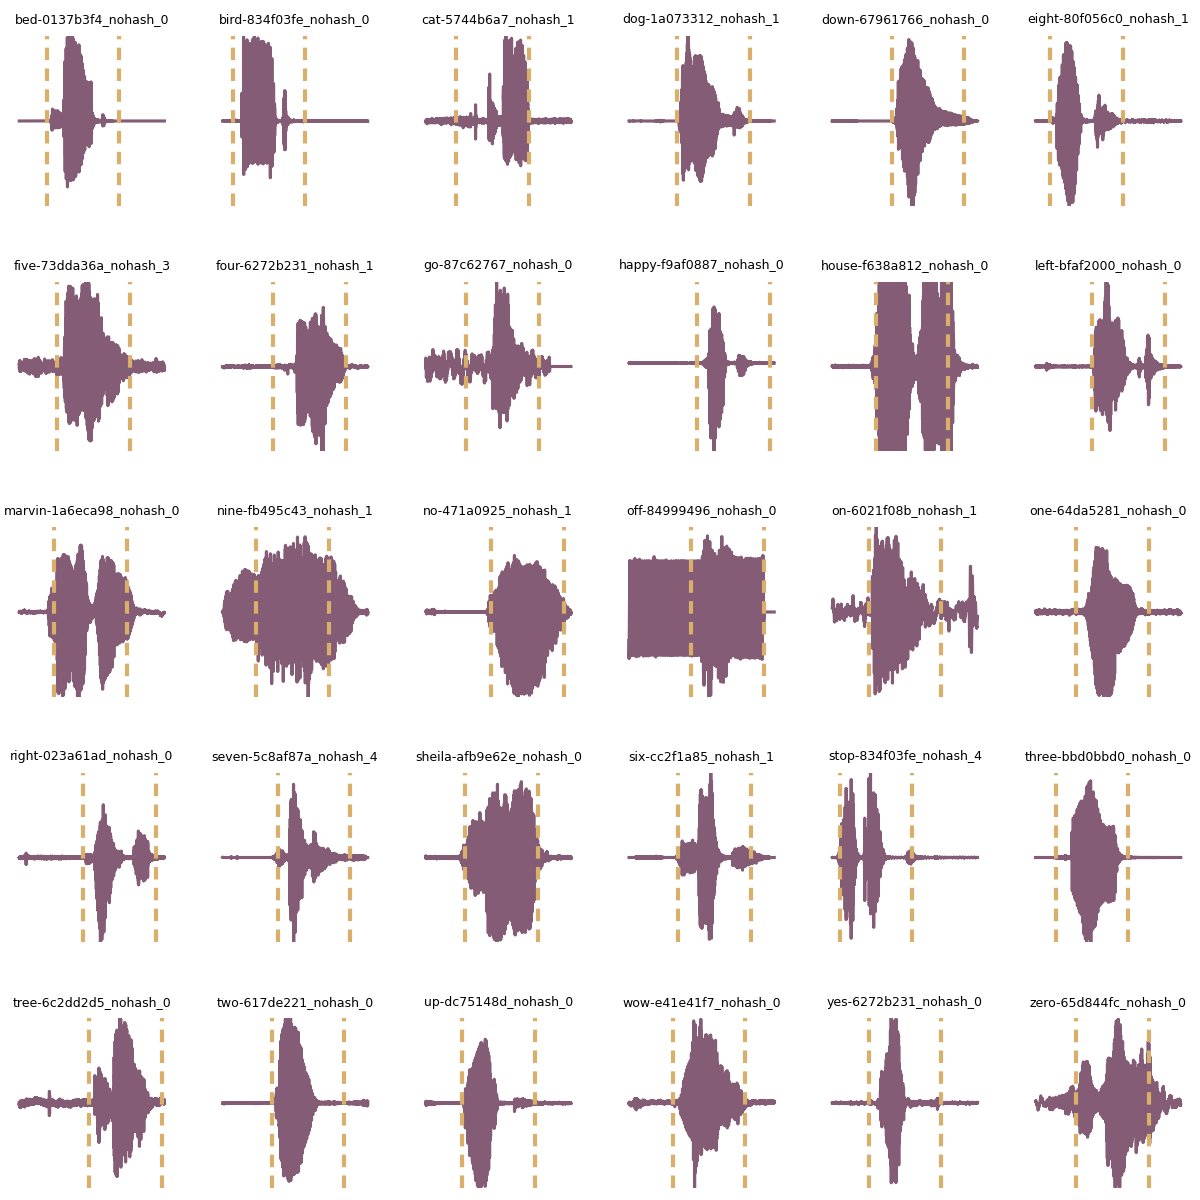
\includegraphics[width=0.65\textwidth]{./5_exp/figs/exp_dataset_wav_grid_c30}
  \caption{One random sample of each individual speech command in the speech command dataset in normalized raw audio format.}
  \label{fig:exp_dataset_wav_grid_c30}
\end{figure}
\FloatBarrier
\noindent

%It has to be mentioned, that it is wonderful, that a dataset for simple key word spotting on speech commands with this amount of diversity and free of access under the creative common license exist.

